\chapter{Usability}
\label{Usability}

This chapter will give a brief definition of what usability is, and how user tests can help us improve it. Since are applications are targeted towards both children and adults, we will give a description of how the usability tests for these gorups will differ. We will also explain how the user testing is performed at \ldots

\section{What is usability?}
There are many ways to describe usability. 

The International Organization for Standardization(ISO) has a definition of the term usability [insert reference from bibliography]: 

Extent to which a system, product or service can be used by specified
users to achieve specified goals with e↵ectiveness, efficiency
and satisfaction in a specified context of use.

The same document defines the context of use as:

Users, tasks, equipment (hardware, software and materials), and
the physical and social environments in which a product is used.

These definitions covers how the system is used, the user's thoughts about the use and the context of the system. This can be broken further down into several subgoals in order to achieve better usability, and to give us a better insight on what usability is. 
These subgoals are:

\begin{enumerate}
\item{How precise is the user able to perform a task using the application?}
\item{How much resources(for example time, or number of tries) was used to perform the given task using the application?}
\item{How many errors occurred?}
\item{Did the user find the use satisfactory?}
\end{enumerate}

User-centered design is a way of designing with the user in mind. By using this technique these goals are achieveable. User-centered design is about getting feedback from the users during the design and development process. Always thinking about how the user would solve this problem, and consolidate the users when in doubt is a fundamental part of user-centered design. The user's opinion is the measure of how good the system performs and the user's feedback defines how you score on usability. [Should have reference]

\section{How to test usability}
There are many ways to create a good user experience. Having knowledge of expert opinions is always a good idea, and using user-centered design techniques are also a wise way to go. According to SOME PERSON [Insert Reference] developers should get feedback from users by users tests at different stages of the development. According to SOME PERSON [Insert reference], having a user-centered approach will help the developers to address the weakest parts of their system, and give feedback on design decisions. 

A user-centered design can be done in many different ways, at different stages of the product lifecycle [Insert reference], as shown in Table \ref{table:designduringlifecycle}:

\begin{table}[H]
\begin{tabular}{|p{5cm} | p{5cm} | p{5cm} |}
\hline
\textbf{Method} & \textbf{Purpose} & \textbf{Phase of the project lifecycle} \\ \hline
Background interviews and questionnaires & To collect data and to understand the user better & When starting the project \\ \hline
Focus groups & Discover design issues and recieve feedback & At early stage \\ \hline
On-site observation & To both collect information of the context the system will be used in, and find the basic problems the users have & At early stage \\ \hline
Role playing / simulations & Will give a broader understanding of what the user expects from the system & Early to mid stage of the project \\ \hline
Automated evaluation & Gives feedback on deviations from standards or best practices. This method exclude actual users, but are based on well tested principles & Mid to end of the project \\ \hline
Usability testing & To measure the usability of your system and provide feedback on very specific elements that are badly designed & Abras [insert reference] says it should be at the end of the project, while others[insert references] thinks it should be done in iterations throughout the project. \\ \hline
Interviews and questionnaires & Gives a qualitative measurement of how good or bad the system is & End of the project \\ \hline
\end{tabular}
\caption{Methods of user-centered feedback}
\label{table:designduringlifecycle}
\end{table}

The purpose of this project is to test an existing system, improve the existing product and plan an extensive testing of the improved product. We will focus mainly on WHAT WHAT WHAT?

\paragraph{Usability Testing}
The purpose of usability testing is to increase the usability of a system. At the same time, performing these usability tests can save the developers some time and reduce the cost of the project by removing errors and poor design at an early stage [Insert reference].

The usability testing can be performed in different ways [Insert reference]. At early stages of the project, low-fidelity prototypes are a good option since they will provide feedback and take proportionatelly little time to make, making it easier to have more iterations of testing. The different testing methods include a potential user of the system performing tasks to provide real data. Observing and recording each usability test can help the developers to analyze their system, and correct the flaws [insert reference]. 

Before starting the usability tests, the developers should set goals planning what they want to know about the system[Insert reference]. This will ensure that the purpose of the test is fulfilled. The developers should then plan tasks according to the desired results. These tasks should allow the user to explore the system, or the parts the developers want to test, giving the test person some time per task, in order to not stress the test person [Insert reference]. 

After planning the test, the test should be run on a number of different test persons. From figure \ref{figure:numberoftests}, you can see that as the number of participants increases, the number of undetected errors decrease. 

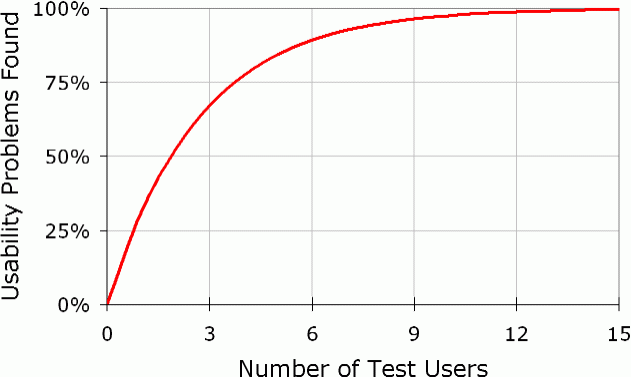
\includegraphics{Thesis/Pictures/numberoftests}


\section{How to test usability on children and toddlers}
While usability testing on children and toddlers have the same basic approach as testing on adults, there are many more precautions to be followed. 
Hanna, Risden and Alexander[insert reference] lays out some of these precautions. They recommend not using children that are skilled with computers, since they may find the tasks to easy and won't give useful data. 
Since children these days have a higher skill with computers thanks to the invasion of tablets and smartphones [insert reference?], this may not as much of a concern. 

Since our application is targeted towards children suffering from Asthma, we want to test the system on children suffering from Asthma in addition to children from the same age group, not suffering from Asthma. These children will most certainly have a different approach to the system and may give different feedback.

THIS NEEDS MORE WORK.